\chapter{Assessing European Preparedness for Cyber Warfare: A Comparative Analysis of France, Estonia, Germany, and the Netherlands}


\section{Introduction}
xxx

\section{France}

This section offers a comprehensive exploration of France's cyber defence strategy, meticulously outlined in the Strategic Review of Cyber Defence (February 2018). By dissecting key components such as operational chains, governance structures, and specific doctrines, we aim to uncover the interconnected layers that constitute France's resilient stance against evolving cyber threats.

In February 2018, France released a White Paper, signalling a strategic shift in its approach to cyber defence. Beyond a mere enumeration of operational chains and governance bodies, this analysis seeks to unravel the cohesive strategy that guides France's response to the dynamic cyber threat landscape.

France's cyber defence strategy unfolds through four operational chains, each with a distinct role. The Protection Chain, spearheaded by SGDSN and ANSSI, stands as the frontline defence for national security during cyberattacks. Complementing this, the Military Action Chain provides the President with the authority to deploy cyber warfare in the interest of national defence. Simultaneously, the Intelligence Chain focuses on attributing cyberattacks, while the Judicial Investigation Chains involve law enforcement in the aftermath of cyber-related crimes \autocite{sgdsn_2018_strategic, anssi_2022_le}.

\begin{figure}[H]
    \centering
    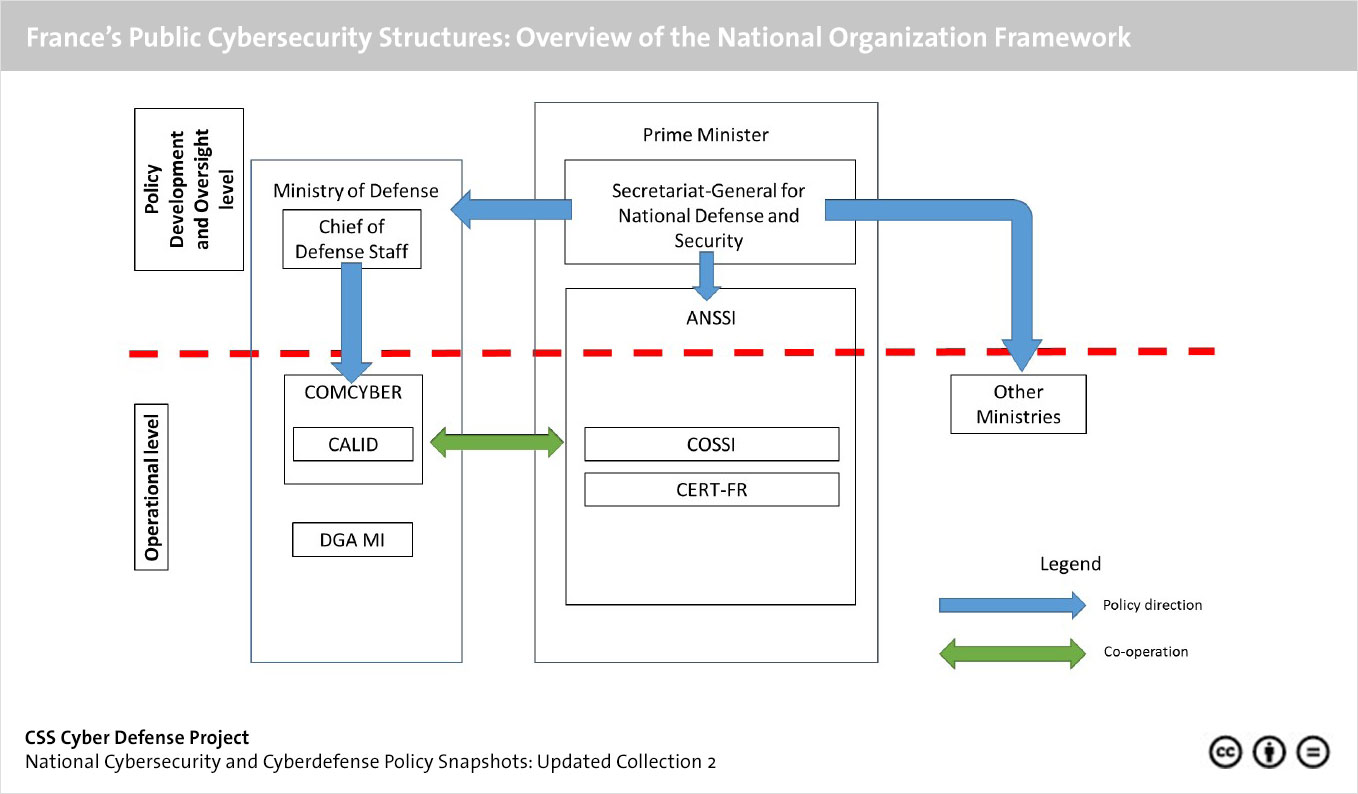
\includegraphics[width=1\textwidth]{Images/france.jpg}
    \caption{\textit{France Cyber Structure}}
        \source{Source: \autocite{sdewar_2018_national}}
    \label{fig:france}
\end{figure}

\textbf{Governance and Crisis Management}: Beyond the operational facets, France has meticulously crafted a governance structure to manage cyber crises. The Cyber Defence Management Committee, Cyber Defence Steering Committee, and Cyber Crisis Coordination Centre collectively orchestrate a harmonized response. The Permanent Cyber Posture (PPC) ensures an uninterrupted 24/7 defence, reflecting a commitment to proactive cyber defence. This interplay of structures and strategies exemplifies a holistic approach to cyber resilience.

\begin{table}[h]
\centering
\renewcommand{\arraystretch}{1.5} % Adjust row height
\caption{Actions Taken by France in Power Instrument \& Capabilities}
\begin{tabular}{>{\raggedright}p{4cm} p{11cm}}
\toprule
\textbf{Power Instrument Capabilities} & \textbf{Actions Taken by France} \\
\midrule
\textbf{Political} & \\
\hspace{0.2cm} Deterrence & No public available information. \\
\hspace{0.2cm} Political Alliances & Actively engages in political alliances for collective cyber defense efforts (Strategic Review of Cyber Defense). \\
\hspace{0.2cm} Involvement of Private Sector & Collaborates with the private sector, emphasizing control over offensive actions and corporate responsibility. Encourages greater private sector control of offensive actions in cyberspace (Strategic Review of Cyber Defense. \\
\hspace{0.2cm} Awareness Campaigns & Conducts awareness campaigns targeting SMEs and public administrations (LID). \\
\midrule
\textbf{Informational} & \\
\hspace{0.2cm} Intelligence Gathering & Actively engages in intelligence gathering to attribute cyberattacks. Conducts information warfare through the Influence Computer Control (L2I) doctrine, focusing on military operations outside the national territory (L2I). \\
\midrule
\textbf{Economical} & \\
\hspace{0.2cm} Protect Critical Infrastructure & Implements measures to safeguard critical infrastructure from cyber threats (Strategic Review of Cyber Defense & SIIV). \\
\hspace{0.2cm} Invest in Skills and Infrastructure & Allocates resources for skill development and cyber infrastructure enhancement. Addresses the challenge of human resources through the Military Program Law 2019-2025 (L2I). \\
\midrule
\textbf{Military} & \\
\hspace{0.2cm} Integration of Cyber-Kinetic (C\&C) & No public available information . \\
\hspace{0.2cm} Use of Preventive (Offensive) Attacks & Adopts offensive cyber measures as preventive actions for national defense (LIO). France's COMCYBER oversees the military cyber offensive capacity, emphasizing the need for political, legal, and military risk evaluations in all phases of operations (LIO). Adopts a public position when necessary for political discourse and to differentiate from clandestine actors (LIO). Addresses challenges in accelerating offensive cyber capabilities, HR policies, training, and convergence with EU partners (LIO). \\
\bottomrule
\end{tabular}
\end{table}


\textbf{Defensive Cyber Warfare Policy (LID)}: The Defensive Cyber Warfare Policy (LID) serves as the linchpin of France's defensive capabilities. Beyond a mere list of missions, LID embodies a strategy of awareness, probability assessment, protection enhancement, detection, reaction, and attribution. The interdependence between these missions showcases a holistic approach to safeguarding national interests. Moreover, the emphasis on collaboration, exemplified by the Network and Information Systems Directive (NIS) and its updated version (NIS2), emphasizes the importance of unified efforts between electronic communication operators, web hosts, and national entities. Local level involvement through coordination forums further cements the idea of a collective defence \autocite{ministredesarmes_2019_politique}.

\textbf{Offensive Cyber Warfare Doctrine (LIO)}: In tandem with defensive measures, France has integrated offensive capabilities within its overall military strategy through the Offensive Cyber Warfare Doctrine (LIO). COMCYBER, operating under the Chief of Staff of the Armed Forces, oversees the orchestration of LIO. By acknowledging the necessity for political, legal, and military risk evaluations, France strikes a delicate balance between secrecy and transparency. The democratic nature of the state guides decisions on the disclosure of LIO actions \autocite{ministredesarmes_2019_lments}.

\textbf{Influence Computer Control (L2I)}: Expanding beyond national borders, France recognizes the importance of information warfare through the Influence Computer Control (L2I). Executed by CYBERCOM, L2I operations aim to detect and counter information attacks, gather intelligence, and engage in deception operations. Challenges, such as the investment in human resources, are met head-on through the Military Program Law 2019-2025, allocating resources for cyber fighters and acknowledging the financial commitment needed \autocite{ministredesarmes_2021_lments}.

France identifies private companies or public bodies that are of vital importance. The \textit{Secteur d'activité d'importance vital} applies to these, a provision which raises the level of security in the event of an attack, including cyberattacks. Due to the increase in cyberattacks, the provision has been transformed specifically for vital information systems (making information systems a separate category of cyber infrastructure). To date, more than 200 entities have been labelled as such with the obligation to notify any incident, as well as apply more stringent crisis prevention and management measures \autocite{anssi_2022_le}.

In conclusion, France's cyber defence strategy is a tapestry woven with interconnected threads, each playing a crucial role in ensuring national cybersecurity. By delving beyond the surface enumeration of strategies, this analysis unravels the symbiotic relationship between operational chains, governance structures, and specific doctrines. In an era of evolving cyber threats, France's adaptive and integrated approach stands as a model for nations navigating the complex landscape of digital security. Furthermore, France has increased its awareness and cyber capabilities even before the War in Ukraine, anticipating strategies on the involvement of public sector in the cyber defence and the use of offensive attacks in their doctrine. However, no public available information for the integration of cyber and kinetic weapons were found. 

\section{Estonia}
Estonia experiences with cyberattacks have shaped not only its own strategy but also became a successful model of how to exploit security vulnerabilities to improve its readiness to counter future attacks. After 2007, Estonia have developed a multifaced cyber strategy, an outcome from a continuous learning and development of proactive defence measures. 

Unlike the other countries analysed in this dissertation, Estonia is more familiar with a real threat that combines kinetic and cyber operations from non-state actors (supported from Russia). In this regard, the National Security Concept published in 2017 highlight that Estonia applies measures to guarantee the digital continuity of the state even in situations where it has lost the control over its territory \autocite[16]{republicofestonia_2017_national}. For a small state like Estonia, the synergy between the private sector, the civil society and the State becomes a priority.  

As well as in the previous analysis, the main challenge that Estonia must tackle regards the skill and specialization. Even the flexibility of being a small country helps professionals to connect with each other and create communities which are valuable in the cyber domain, this approach to the crisis management could not be sustainable due to increase complex of technology risks.  

Estonia is actively involved in the international cooperation in the cyber domain. It hosts the Cooperative Cyber Defence Centre of Excellence (CCDCOE), a NATO-accredited centre for cybersecurity and cyber defence. In fact, Tallinn CCDCOE hosts the most important NATO cyber exercises, such as the Cyber Coalition and Locked Shields. The alignment with allied military presence, particularly NATO's Enhanced Forward Presence (eFP), underscores the need for evolving cooperation mechanisms and procedures to collectively address cyber threats. Estonia aims to establish a comprehensive approach, encompassing political, legal, and technical dimensions, to attribute cyber-attacks, participate in deterrence efforts, and collaborate with like-minded countries in cyber defence frameworks \autocite{ministryofeconomicaffairsandcommunication_2019_cybersecurity}. 

The small Baltic country has also bilateral cyber exercise such as Baltic Blitz 23 with United Stated, as well as joint defensive operations with the USCYBERCOM\footnote{ Information about this operation were published by the US Cyber Command on their website: https://www.cybercom.mil/Media/News/Article/2433245/hunt-forward-estonia-estonia-us-strengthen-partnership-in-cyber-domain-with-joi/}. While Estonia official document do not mention the cyber offensive capabilities of their military, the Baltic State has been a central player in hosting NATO Crossed Swords, a redteamming exercise with the aim to explore the kinetic-cyber synergies in a wartime scenario \footnote{ Even if exercises like that are under exceptional secrecy, local media offers useful insights: https://news.err.ee/1608427058/offensive-cyber-operations-exercise-kicks-off-in-estonia}. 

\begin{figure}[H]
    \centering
    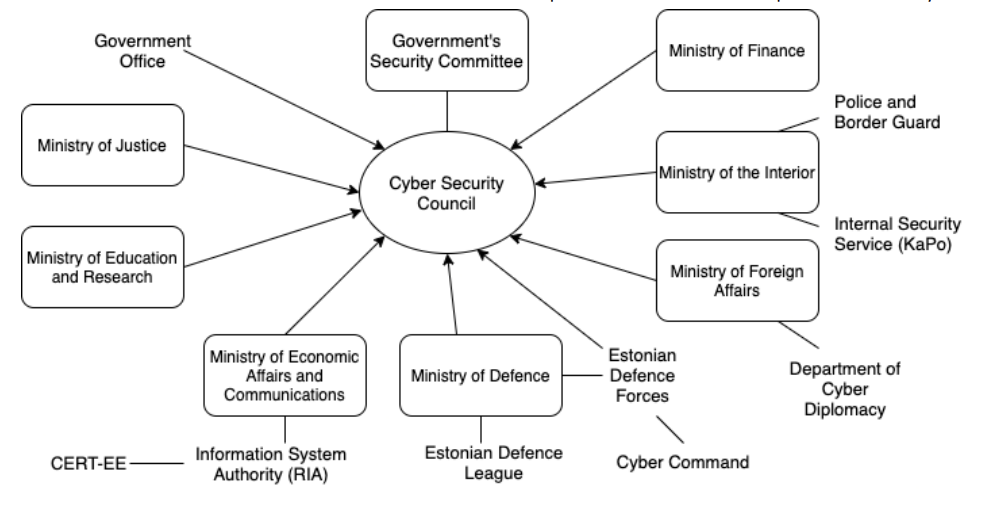
\includegraphics[width=1\textwidth]{Images/estonia.png}
    \caption{\textit{Estonia Cyber Structure}}
        \source{Source: \autocite{kohler_2020_cyberdefense}}
    \label{fig:estonia}
\end{figure}

From the military perspective, the Cyber Command, which become operation in 2018, have the task to carry out cyber operations and to provide cyber defence. The Cyber Command subdivisions include \autocite{defenceforces_2023_cyber}: 
\begin{itemize}
    \item ICT centre: develop the defence architecture of military forces, as well as coordinating the development in the technology domain. 
    \item Cyber Information Operation Centre: prepare the reserve units and active planning of cyber operations and defence.
\end{itemize}

Estonia represents a unique case in which a civil cyber army is officially recognized as part of the Estonian Armed Forces. The country's cyber civil defence force, which is integrated into the Estonian Defence League, is dedicated to enhancing national cyber resilience. Members of this unit typically comprise IT professionals, programmers, and individuals possessing expertise in cybersecurity. The cooperation between civil society and the state is palpable in this framework. By involving IT experts and cybersecurity specialists from outside traditional military establishments, Estonia fortifies the bond between the government and the public, thereby cultivating a shared responsibility for national cybersecurity.

Estonia embrace deterrence by denial in the cyberspace \autocite{oh_2019_exploring}. The aim is to make it difficult for attackers to achieve their objectives, thereby dissuading them from attempting cyberattacks in the first place. 

For what regards the protection of critical information infrastructure, the Information System Authority (RIA) is the competent authority which encompass the cyber crisis management. Additionally, RIA works with state authorities and businesses that provide essential services to coordinate efforts to avoid and handle cyber emergencies. It also collaborates on civilian-military cyber initiatives with the Defence Forces and Defence League. Moreover, RIA coordinates the national response to significant cyber incidents, which are defined as incidents that jeopardize or negatively impact system security, in compliance with the Emergency Act. Through incident prevention, preparedness planning, and incident response coordination, RIA maintains a state of readiness by utilizing strategies like legislative advancements, security officer network management, and other training efforts. In order to prepare for large-scale cyber incidents, RIA's Incident Response Department regularly conducts risk analyses to evaluate the likelihood and consequences of such events. Depending on the type and extent of the emergency, this preparation may involve working with other cybersecurity departments and pertinent authorities listed in the Emergency Response Plan, such as the Cyber Unit of the Estonian Defence League \autocite{informationsystemauthority_2022_cyber}


\begin{table}[h]
\centering
\renewcommand{\arraystretch}{1.5} % Adjust row height
\caption{Actions Taken by Estonia in Power Instrument \& Capabilities}
\begin{tabular}{>{\raggedright}p{4cm} p{11cm}}
\toprule
\textbf{Power Instrument Capabilities} & \textbf{Actions Taken by Estonia} \\
\midrule
\textbf{Political} & \\
\hspace{0.2cm} Deterrence & Detterence by denial. \\
\hspace{0.2cm} Political Alliances &Actively participates in international cooperation, hosting the Cooperative Cyber Defence Centre of Excellence (CCDCOE), a NATO-accredited center. Engages in bilateral cyber exercises and joint defensive operations with partners like the USCYBERCOM. \\
\hspace{0.2cm} Involvement of Private Sector &  Prioritizes synergy between the private sector, civil society, and the state for comprehensive cybersecurity (National Security Concept 2017:16). \\
\hspace{0.2cm} Awareness Campaigns & Public programs to increase awarness to citizens and private companies. Estonia has a priority to cyber literate itz citizens (Cyberstrategy 2019-2022) . \\
\midrule
\textbf{Informational} & \\
\hspace{0.2cm} Intelligence Gathering & No public available information \\
\midrule
\textbf{Economical} & \\
\hspace{0.2cm} Protect Critical Infrastructure & The Information System Authority (RIA) is the competent authority overseeing cyber crisis management and coordinating efforts with state authorities and businesses to protect critical information infrastructure \\
\hspace{0.2cm} Invest in Skills and Infrastructure &  Challenges related to skill and specialization are acknowledged, and efforts are made to enhance national cyber resilience by involving IT experts and cybersecurity specialists. The Cyber Command subdivisions, including the ICT center and Cyber Information Operation Centre, contribute to skill development and technology domain coordination. \\
\midrule
\textbf{Military} & \\
\hspace{0.2cm} Integration of Cyber-Kinetic (C\&C) &  Cyber exercises such as NATO Crossed Swords, exploring kinetic-cyber synergies in wartime scenarios \\
\hspace{0.2cm} Use of Preventive (Offensive) Attacks & Estonia participate in offensive cyber exericises such as Baltic Blitz 23 \\
\bottomrule
\end{tabular}
\end{table}

In summary, Estonia's response to cyber threats stands as a resilient model shaped by its experiences, particularly the impactful cyberattacks in 2007. This multifaceted strategy reflects a continuous commitment to learning and proactive defence. Unlike its counterparts, Estonia faces a tangible threat, blending kinetic and cyber operations from non-state actors, necessitating measures to ensure digital continuity even in the absence of territorial control.

\section{Germany}

\section{Netherlands}

\section{Comparative analysis}

\section{Conclusion}

